Treffen $\gamma$- oder $\beta$- Strahlen auf Materie, so treten in der Materie Wechselwirkungen auf, die zur Abschwächung der Intensität des einfallenden Strahls führen.
Um wechselwirken zu können müssen die Strahlen auf Atome treffen, welche als Zielscheibe vereinfacht werden. Der Wirkungsquerschnitt kann als Fläche der Ziehlscheibe angesehen werden und ist somit ein Ausdruck der Wahrscheinlichkeit für das Aufreten von Wechselwirkungen.
Die Anzahl der Wechselwirkungen kann als
\begin{align*}
  N=N_0nD\sigma
\end{align*}
angegeben werden. Dabei ist $D$ die Dicke des Materials, $n$ die Anzahl der Materieteilchen pro Volumeneinheit und $N_0$ die Anzahl der Teilchen die pro Zeiteinheit auf das Material treffen.
Die Intensität der Strahlung fällt im Material exponentiell ab.
\begin{align}
  N(D)=N_0\cdot e^{-n_\sigma D}
  \label{eqn:e}
\end{align}
Der Absorptionskoeffizient $n_\sigma$ wird meist als $\mu$ abgekürzt. $n(D)$ beschreibt die Anzahl der zu messenden Aktivität nach der entsprechenden Dicke. Die Ausgangsaktivität wird mit $N_0$ betitelt, wärend $n$ die Anzahl der Telchen im Absorber pro Volumen beschreibt.
n wird folgendermaßen berechnet
\begin{align*}
  n=\frac{\text{z}N_A}{V_{\text{Mol}}}=\frac{\text{z}N_A\rho}{M}
\end{align*}
$z$ ist dabei die Ortnungszahl, $N_A$ die Avogadro-Konstante und $V_\text{Mol}$ das Molvolumen. Das molekulargewicht wird als M abgekürzt und die Dichte als $\rho$.
Im Falle der $\beta$-Strahlung gilt das Absorptionsgesetzt nur für kleine Dicken.
\subsection{$\gamma$-Strahlung}
Ein $\gamma $-Quant wird emittiert, wenn ein angeregter Atomkern in einen energetisch niedrigeren Zustand wechselt. Die Energienivaus sind diskret, daher tritt ein diskretes Linienspektrum auf. Die $\gamma$-Strahlung weist alle Eigenschaften einer elektromagnetischen Welle auf.
Die Welle kann unterschiedlich mit Materie wechselwirken. Bei einer Annihilation verschwindet das $\gamma$-Quant. Eine inelastische Streuung führt zu einer Richtungsänderung wober ein Teil der Energie an den Stoßpatner abgegeben wird. Eine Richtungsänderung ohne Energieabgabe wird als elastische Streuung bezeichnet.
\begin{figure}[h!]
  \centering
  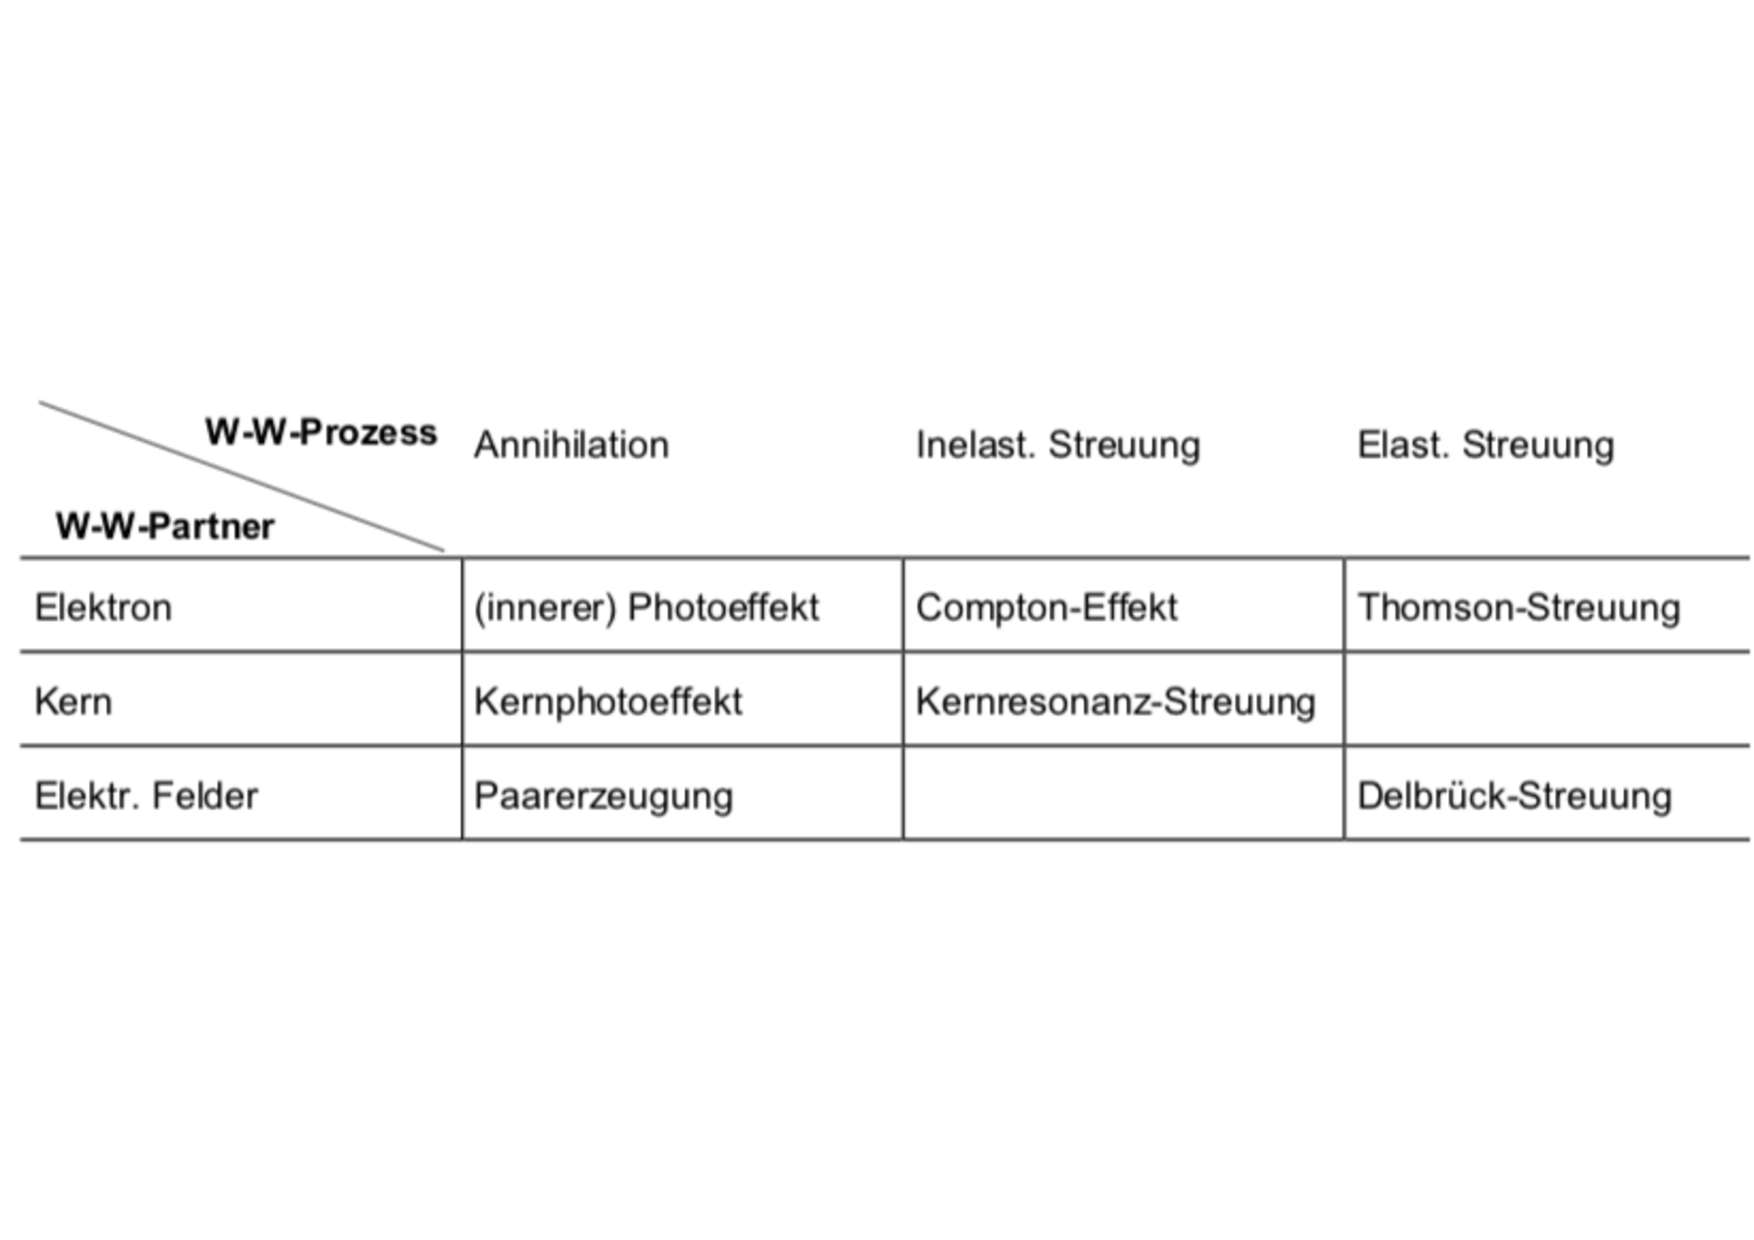
\includegraphics[width=\textwidth]{tabgamma.pdf}
  \caption{Wechselwirkungsarten der $\gamma$-Strahlung \cite{1}}
  \label{fig:Wgamma}
\end{figure}
Die wichtigsten Prozesse sind der Photo-Effekt, der Compton-Effekt und die Paarbildung.
\FloatBarrier
\subsubsection{Photo-Effekt}
Das $\gamma$-Quant geht eine Wechselwirkung mit einem Hüllenelektron ein wobei das Elektron aus seiner Bindung entfernt wird. Das $\gamma$-Quent wird dabei vernichtet, da es seine gesammte Energie an das Elekton abgibt.
Das Elektron hat dann eine kinetische Energie von:
\begin{align*}
  E_{\text{kin}}=h\nu-E_B.
\end{align*}
$h\nu$ ist dabei die Energie des Photons. Die Bindungsenergie es Elektrons wird als $E_B$ angegeben.
Da die Bindungsenergie für das Auslösen eines Elektrons erst überschritten werden muss gibt es eine Energieschwelle unter der der Photo-Effekt nicht funktioniert.
%Frage: es werden als erstes die Elektronen am Atomkern Ausgeschlagen wobei diese die höchste bindungsennergie besitzen. das liegt irgendwie an dem drehimpuls. warum haben wir bei der röntgenemmission gesagt genug ennergie für die nächste schale? wie viel Ennergie wird denn dann gebraucht?
\subsubsection{Compton-Effekt}
Der Compton-Effekt fällt unter die Rubrik der inelastischen Streuung. Ein $\gamma$-Quant wird an einem freien Elektron gestreut und verliert einen Teil seiner Energie.
Durch die diffuse Streuung nimmt die Intensität des $\gamma$-Strahls ab. Der Wirkungsquerschnitt $\sigma_{\text{com}}$ ist gegeben durch:
\begin{equation}
  \sigma_{\text{com}}=2\pi r^2_e\left(\frac{1+\epsilon}{\epsilon}^2\left[\frac{2(1+\epsilon)}{1+2\epsilon}-\frac{\text{ln}(1+2\epsilon)}{\epsilon}\right]+\frac{\text{ln}(1+2\epsilon)}{2\epsilon}-\frac{1+3\epsilon}{(1+2\epsilon)^2}\right).
\label{eqn:sigma}
\end{equation}
$r_e$ beschreibt den klassischen Elektronenradius und wird als $r_e=\SI{2,82e-15}{m}$ angenommen. Das Verhältnis der Quantenenergie $E_\gamma$ zu der Ruheenergie wird als $\epsilon$ bezeichnet.
Der Absorptionskoeffizient berechnet sich dann über:
\begin{align}
  \mu_{\text{com}}= \frac{Z N_{\text{A}} \rho \sigma_{\text{com}}}{M}.
  \label{eqn:koeff}
\end{align}
\subsubsection{Paarerzeugung}
\begin{figure}[h!]
  \centering
  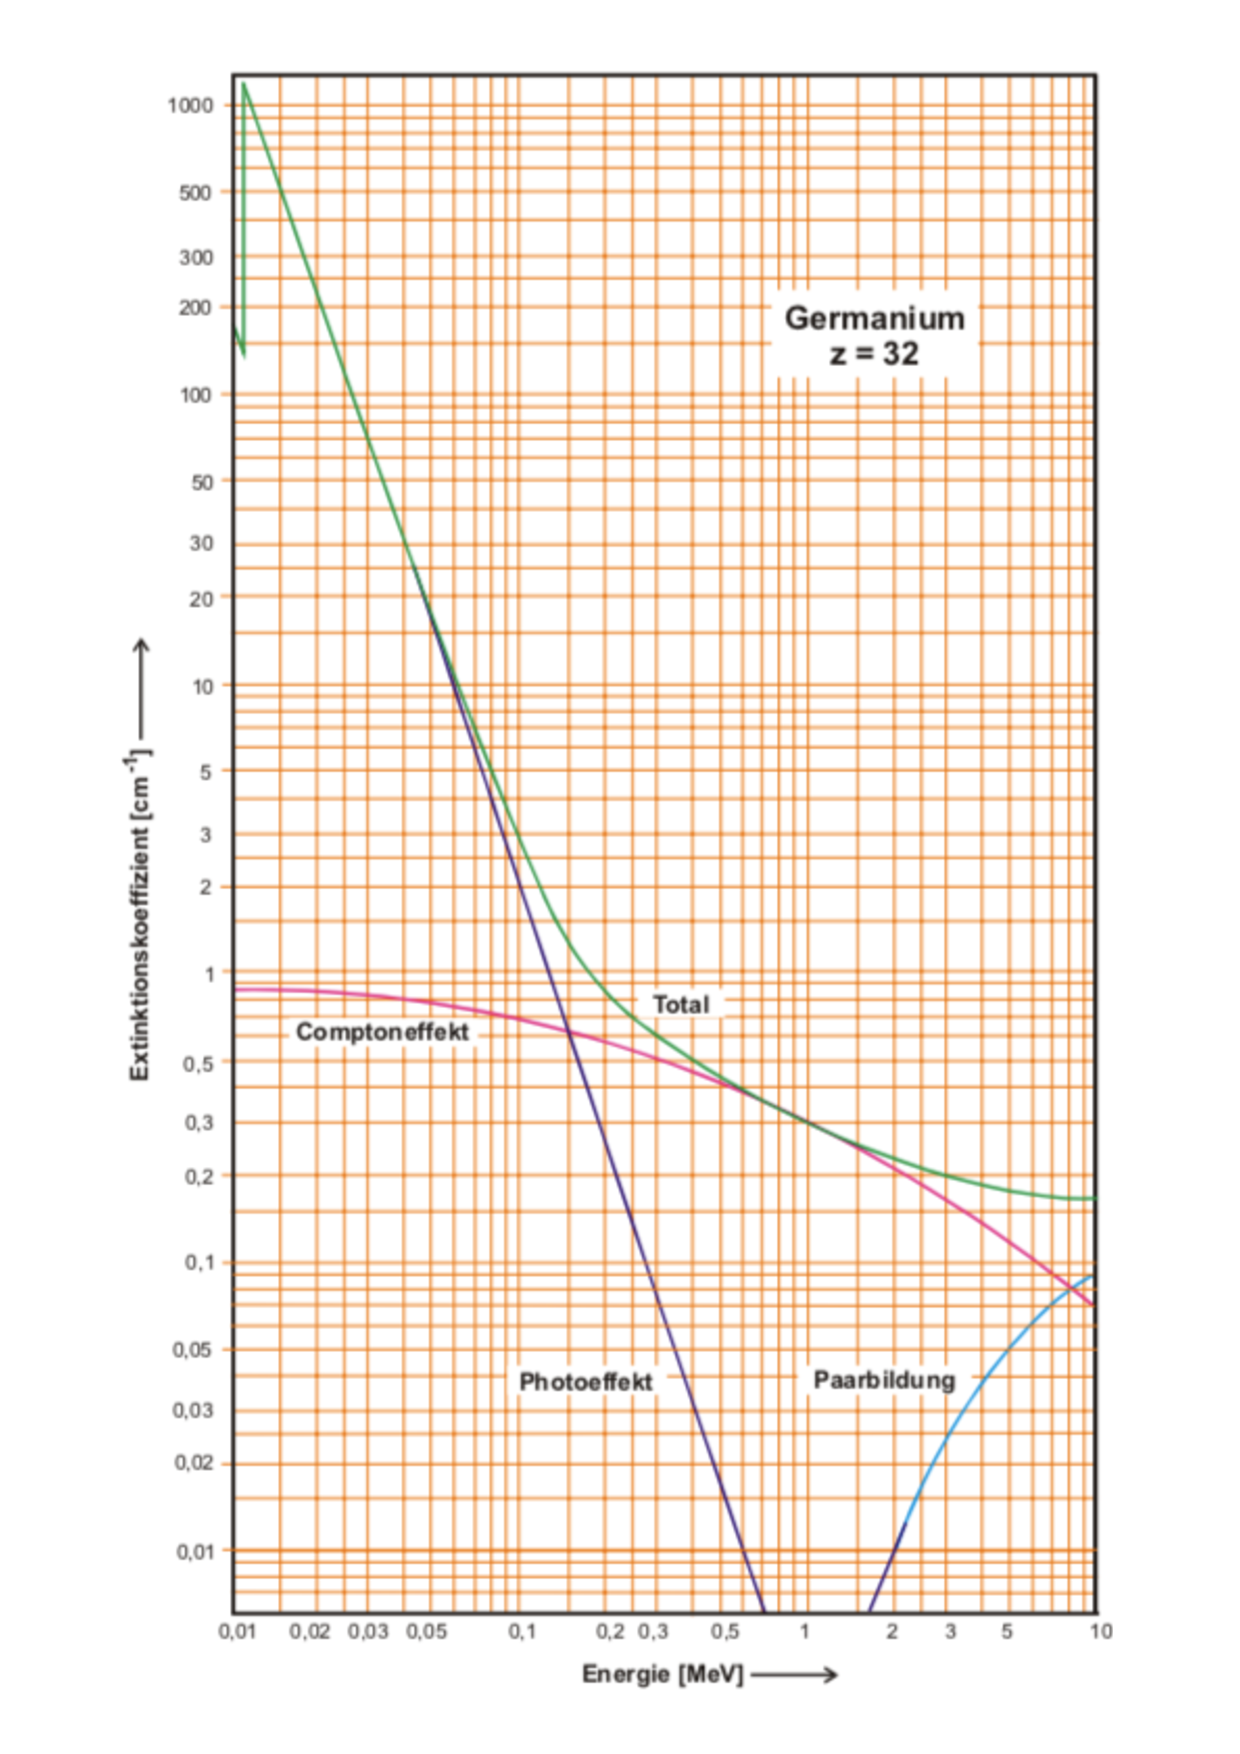
\includegraphics[width=0.5\textwidth]{abbs.pdf}
  \caption{Absorptionskoeffizient in Abhängigkeit von der Energie für Germanium \cite{1}}
  \label{fig:abbs}
\end{figure}
Zu Paarbildung kommt es, wenn die Energie des $\gamma$-Quants mindestens doppelt so hoch
ist, wie die Ruhemasse eines Elektrons. Unter Annihilation des Photons kommt es zur Bildung eines Elektrons und eines Positrons.
Für den Vorgang muss sowohl die Energieerhaltung als auch die Impulserhaltung erfüllt sein. Daher muss die absorbierte Energie vom Betrag über $2m_0c^2$ liegen.\\

Im Wesentlichen überlagern sich die drei genanten Effekte beim Durchgang eines $\gamma$-Strahls durch Materie und sind somit an der Bildung des Absorptionskoeffizienten verantwortlich. Für niedrige Quantenenergieen dominiert der Photoefekt. Bei größer werdender Energie ist die Paarbildung der ausschlaggebende Effekt. Zwichen den beiden spielt der Compton-Effekt ein große Rolle.
Diese Zusammenhänge sind in der Abb. \ref{fig:abbs} verdeutlicht.

\FloatBarrier
\subsection{$\beta$-Strahlung}
Zur $\beta$-Strahlung kommt es, wenn ein Neutron oder ein Proton eines Atomkerns zerfällt.
\begin{align*}
  n\to p+\beta^-+\overline\nu_e\\
  p\to n+\beta^++\nu_e
\end{align*}
Im folgenden wird nur der Zerfall eines Neutrons betrachtet.
Das Neutron zerfällt in ein Proton und ein Antineutrino $\overline\nu_e$. Das ebenfalls entstehende Elektron besitzt eine hohe kinetische Energie und wird als $\beta$-Strahlung bezeichnet.
Die durch den Zerfall freiwerdende Energie verteilt sich statistisch auf das Elektron und das Antineutrino, wie in Abbildung \ref{fig:emiss} zu sehen. Das hat zur Folge, dass das $\beta$-Spektrum kontinuierlich ist.
Die maximale Energie $E_{\text{max}}$ die ein Elektron haben kann, ist gleich der gesamten Energie die beim Zerfall frei wird.
\begin{figure}[h!]
  \centering
  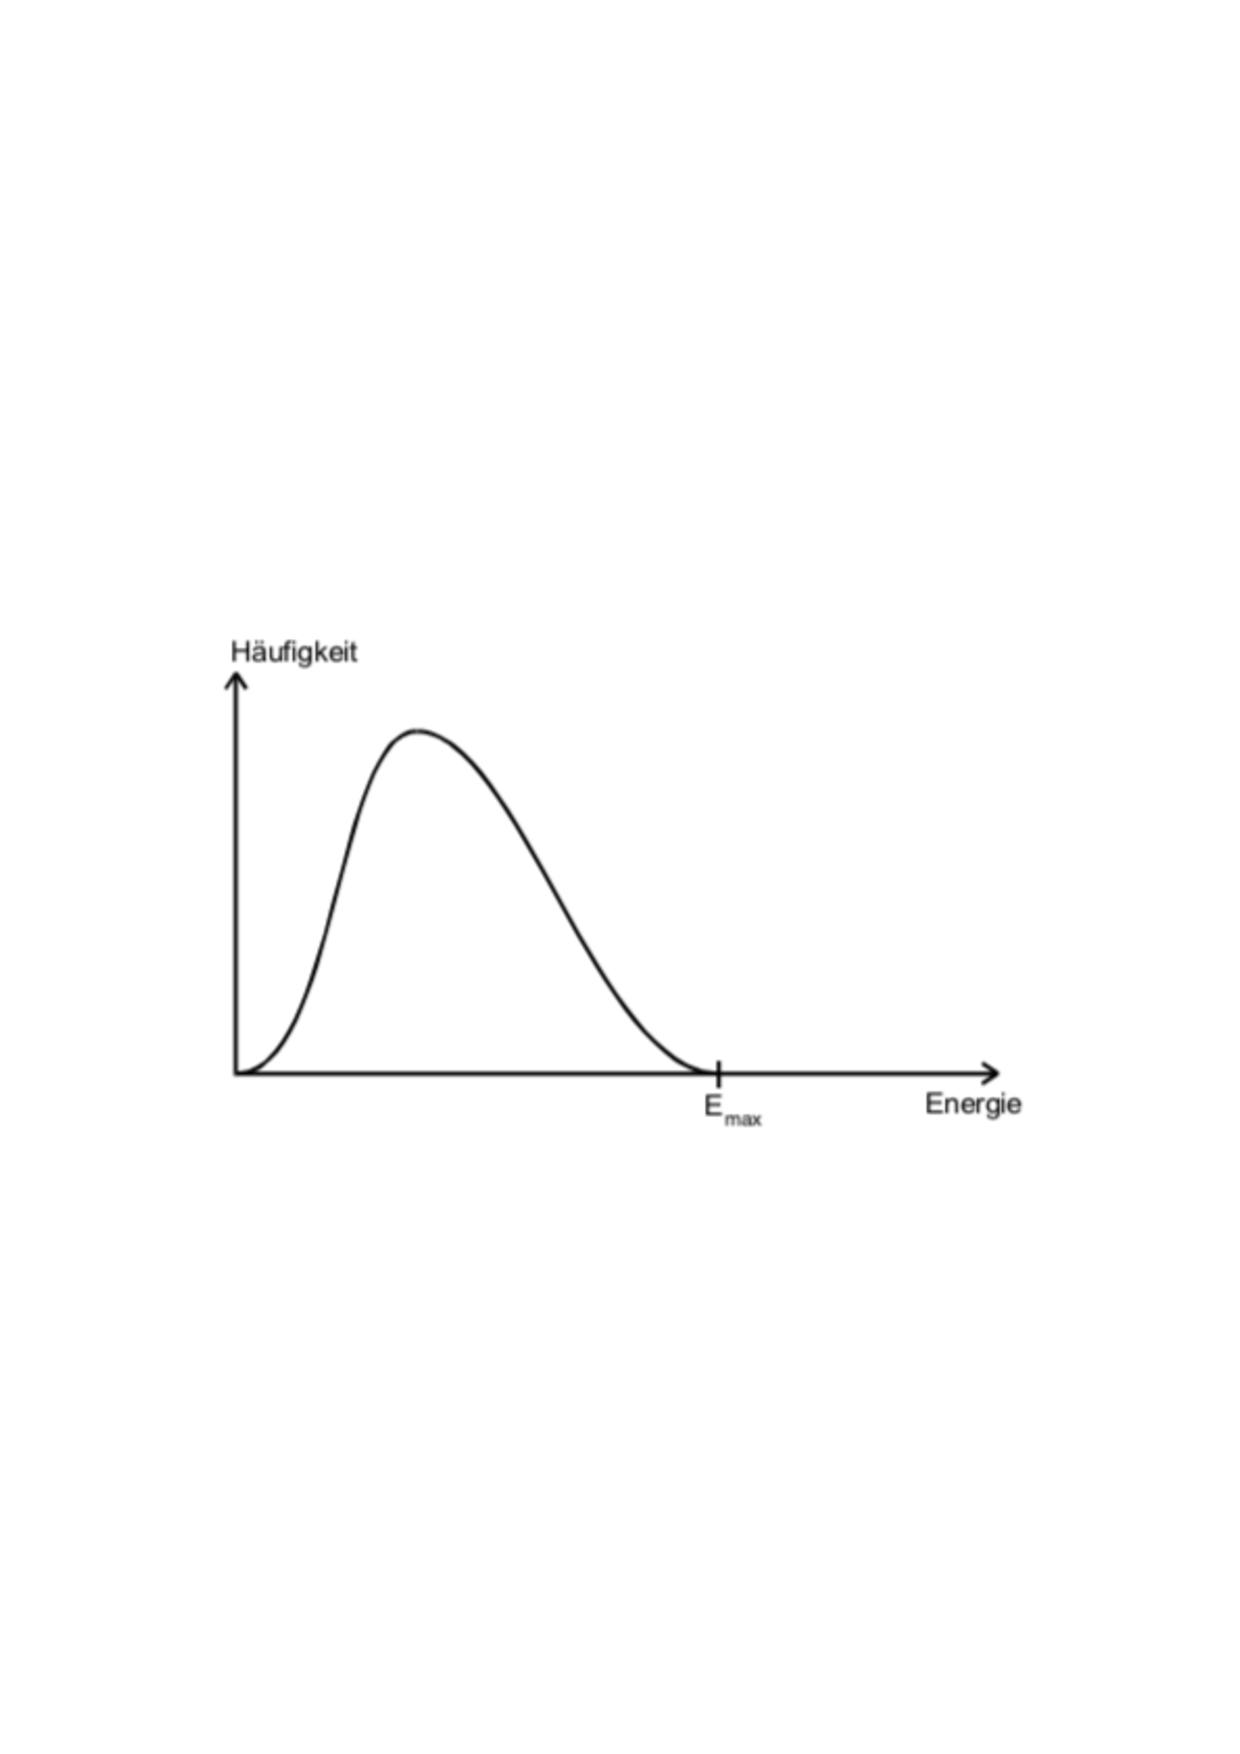
\includegraphics[width=\textwidth]{Emiss.pdf}
  \caption{Emmissionsspektrum eines $\beta$-Strahlers \cite{1}}
  \label{fig:emiss}
\end{figure}
Beim Zerfall muss die Energie-, Impuls-und Drehimpulserhaltung gelten.
Der Durchlauf von $\beta$-Strahlung durch Materie ist im wesentlichen von drei Prozessen bestimmt. Es treten jeweils eine Vielzahl von Wechselprozessen auf.
\FloatBarrier
\subsubsection{Elastische Streuung am Atomkern}
Die Elektronen werden unter einem sehr geringen Energieverlust vom Coulomb-Feld des Kerns abgelenkt.
Durch die Ablenkung wird der Strahl aufgefächert und verliert so an Intensität.
Desweiterern bewirkt die Streuung eine Verlängerung des Weges der Elektronen im Material und somit zu einer höheren Warscheinlichkeit für Wechselwirkungen.
\subsubsection{Inelastische Streuung am Atomkern}
Die $\beta$-Teilchen werden im Coulomb-Feld der Kerne beschleunigt.
Durch die Beschleunigung geben die Elektronen Energie in Form von elektromagnetische Strahlung ab.
Die abgegebene Strahlung wird als Bremsstrahlung bezeichnet.
\subsubsection{inelastische Streuung an Elektronen}
Die $\beta$-Teilchen ionisieren das Absorbermaterial und regen es an. Da die dabei abgegebene Energie sehr gering ist kann das $\beta$-Teilchen eine Vielzahl von Wechselwirkungen eingehen.\\\\\\


Für Natürliche $\beta$-Strahlen, wie im Experiment verwendet, gilt für geringen Schichtdicken ein Absorptionsgesetz nach \eqref{eqn:e}.
Nähert sich die Schichtdicke der maximalen Reichweite der Teilchen kommt es zu starken Abweichungen, da die Untergrundstrahlung einen immer größeren Einfluss auf die Messung nimmt.
Überschreitet die Schichtdicke die maximalen Reichweite tritt nur noch Untergrundstrahlung auf.
Die zu Absorptionskurve ist in der Abb.\ref{fig:Ab} dargestellt.
Über diese ist es möglich die maximale Reichweite $R_{\text{max}}$ zu bestimmen.
\begin{figure}[h!]
  \centering
  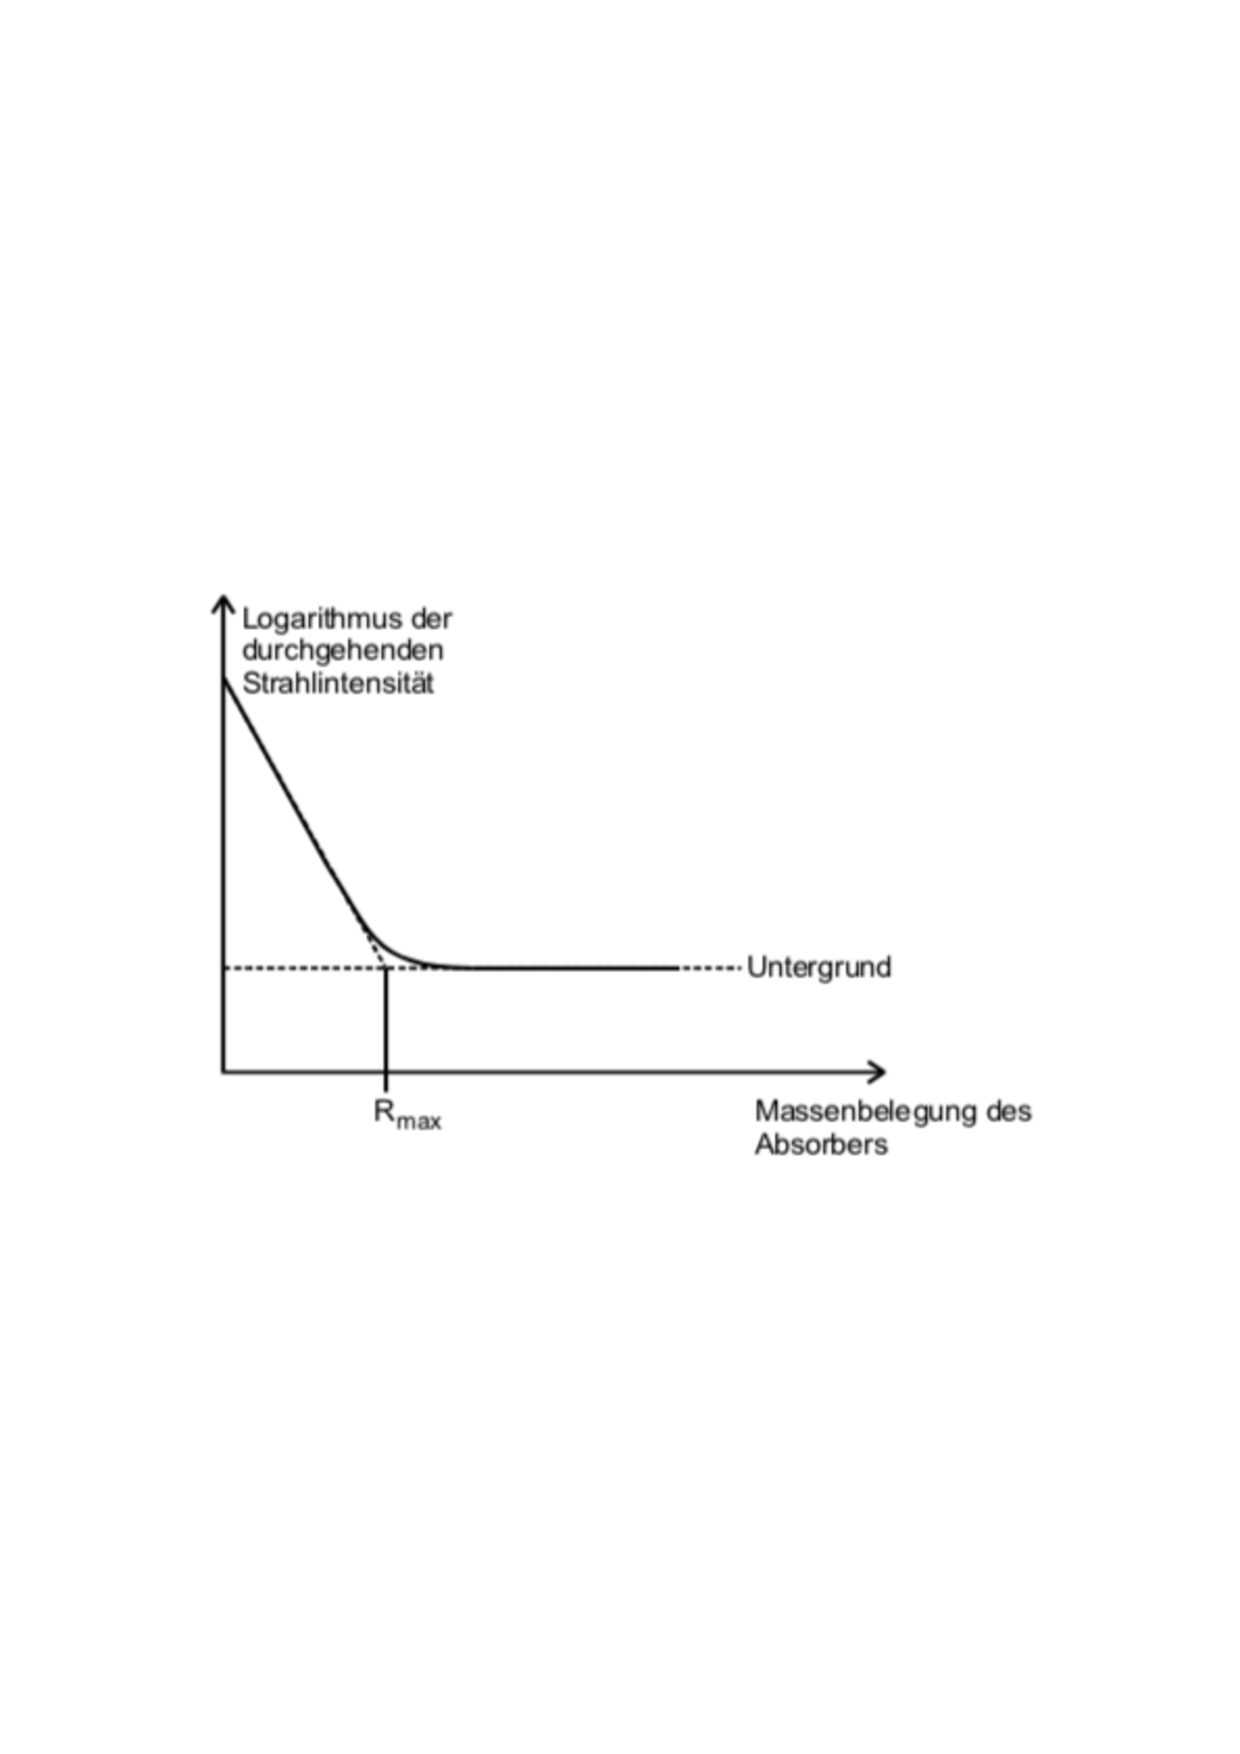
\includegraphics[width=\textwidth]{Ab.pdf}
  \caption{Absorptionskurve für einen natürlichen $\beta$-Strahler \cite{1}}
  \label{fig:Ab}
\end{figure}
Hier wird jedoch nicht die Dicke D des Absorbers sondern die Massenbelegung R aufgetragen. Diese hängen wie folgt zusammen:
\begin{equation}
  R=\rho D
  \label{eqn:massenbelegung}
\end{equation}
Da $R_{\text{max}}$ größtenteils durch die energiereichsten Elektronen bestimmt wird, kann so auf die $E_{\text{max}}$ geschlossen werden.
Die verwedete Formel wurde nur empirisch bestimmt.
\begin{align}
  E_{\text{max}}= 1,92\sqrt{R^2_{\text{max}}+0,22R_{\text{max}}}[MeV]
\end{align}
$E_{\text{max}}$ hat eine Größenordnung von $\SI{10e6}{eV}$.
\FloatBarrier
